\documentclass{beamer}
\usepackage{beamerthemeshadow}

%\documentclass{article}
%\usepackage{beamerarticle}
%\usepackage{graphicx}

\usepackage{verbatim}
\usepackage{lastpage}
\usepackage{xcolor}
\usepackage{pgf}
\usepackage{colortbl}

\newcommand{\bi}{\begin{itemize}}
\newcommand{\ei}{\end{itemize}}
\newcommand{\be}{\begin{enumerate}}
\newcommand{\ee}{\end{enumerate}}
\newcommand{\bd}{\begin{description}}
\newcommand{\ed}{\end{description}}
\newcommand{\prbf}[1]{\textbf{#1}}
\newcommand{\prit}[1]{\textit{#1}}
\newcommand{\beq}{\begin{equation}}
\newcommand{\eeq}{\end{equation}}
\newcommand{\bdm}{\begin{displaymath}}
\newcommand{\edm}{\end{displaymath}}

\newcommand{\ft}[1]{
  \frametitle{\begin{tabular}{p{4.2in}r} \textcolor{white}{#1} & \small{\insertframenumber / \inserttotalframenumber} \end{tabular}}
  %\frametitle{#1}
  \setbeamercovered{transparent=18}
}

\newcommand{\stepinv}{\setbeamercovered{invisible}}
\newcommand{\stopinv}{\setbeamercovered{transparent=18}}
\newcommand{\uncoverinv}[1]
{
  \setbeamercovered{invisible}
  \uncover<+->{#1}
  \setbeamercovered{transparent=18}
}
\newcommand{\ans}[1]{\textcolor{blue}{#1}}
\newcommand{\ansinv}[1]
{
  \setbeamercovered{invisible}
  \uncover<+->{\textcolor{blue}{#1}}
  \setbeamercovered{transparent=18}
}
\newcommand{\setinv}{\setbeamercovered{invisible}}
\newcommand{\setvis}{\setbeamercovered{transparent=18}}
\newcommand{\centerpic}[2]
{
  \begin{center}
  \includegraphics[#1]{#2}
  \end{center}
}
\newcommand{\h}[1]{\hat{#1}}
\newcommand{\ds}{\displaystyle}

%\definecolor{light}{rgb}{1.0,0.33,0.33}
\definecolor{light}{rgb}{0.9,0.9,0.0}
\newcommand{\hl}[1]{\alt<#1>{\rowcolor{light}\hspace*{-2.1pt}} {\hspace*{-2.1pt}} }

\definecolor{mycolor}{rgb}{0.9,0.9,0.0}
\usecolortheme[named=mycolor]{structure}

\title{Regime Switching, Learning, and the Great Moderation}
\author[James Murray, Viterbo University]{James Murray\\Dahl School of Business\\Viterbo University}
\date{Friday, March 27, 2009}

\begin{document}

\frame{\titlepage}
%\maketitle
\setcounter{framenumber}{0}

\section{Introduction}
\subsection{Purpose}

\frame
{
  \ft{Purpose}
  \bi
  \item<+-> How much does ``bad luck'' explain changing volatility when adaptive expectations react to suspicions of structural changes.
  \item<+-> \textbf{Great Inflation / Great Moderation:} decade of high inflation and volatility followed by seemingly permanent reduction in macroeconomic volatility.
  \item<+-> Bad luck explanation: changes in volatility is due to \textit{exogenous} changes in variance of structural shocks.
  \item<+-> Adaptive expectations:
    \bi
    \item<+-> Agents do not know reduced form parameters governing evolution of the economy.
    \item<+-> Agents estimate a reduced form VAR(1) by least squares.
    \item<+-> Agents endogenously give more recent observations more weight.
    \ei
  \ei
}

\subsection{Bad Luck}
\frame
{
  \ft{Bad Luck}
  \bi
  \item<+-> Volatile periods were hit with bad shocks.
  \item<+-> Sims and Zha (AER, 2006): evidence points in favor of bad shocks over changes in policy.
  \item<+-> Stock and Watson (2003): improved policy accounts for only small part of volatility slowdown.
  \item<+-> Justiniano and Primiceri (AER, 2008): evidence points in favor of time evolving variance of structural shocks.
  \ei
}

\subsection{Adaptive Expectations}
\frame
{
  \ft{Adaptive Expectations}
  \bi
  \item<+-> Oraphanides and Williams (JEDC, 2005): Monetary authority was optimizing, but mis-informed.
  \item<+-> Primiceri (QJE, 2006): Monetary authority mis-informed, expectations improved with time.
  \item<+-> Milani (JME, 2007): Agents learn, little evidence of difference in policy parameters.
  \item<+-> Milani (2008): Time varying expectations explains time-varying volatility.
  \item<+-> Bullard and Singh (2007): bad luck + Bayesian learning.
  \ei
}

\section{Framework}
\subsection{New Keynesian Model}
\frame
{
  \ft{New Keynesian Model}
  \bi
  \item<+-> Consumer behavior:
    \bi
    \item<+-> Choose consumption and labor to maximize utility.
    \item<+-> Habit formation: utility on consumption depends on past consumption.
    \ei
  \item<+-> Producer behavior:
    \bi
    \item<+-> Intermediate goods are produced with labor in monopolistically competitive markets.
    \item<+-> Intermediate goods subject to Calvo (1983) price friction.
    \item<+-> Price indexation: when not re-optimizing prices, price can adjust according to past inflation.
    \ei
  \item<+-> Taylor (1993) type monetary policy:
    \bi
    \item<+-> Nominal interest rate responds to inflation, expected future output gap, and past interest rate.
    \ei
  \ei
}

\frame
{
  \ft{Optimal Consumer Behavior}
  \uncover<+->{\bdm \begin{array}{c} 
      \tilde{\lambda}_{t} = E_t \tilde{\lambda}_{t+1} + \h{r}_t - E_t \pi_{t+1} - r_t^n, \\ \\
      \tilde{\lambda}_t = \frac{1}{ (1-\beta \eta)(1-\eta)}\left[ \beta \eta  E_t \tilde{y}_{t+1} - (1+\beta \eta^2) \tilde{y}_t + \eta \tilde{y}_{t-1} \right] 
      \end{array}
      \edm}

  \bi
  \item<+-> Variables:
    \bi
    \item<.-> $\tilde{\lambda}_{t}$: marginal utility of income.
    \item<.-> $\tilde{y}_t$: output gap.
    \item<.-> $\h{r}_t$: nominal interest rate.
    \item<.-> $\pi_{t}$: inflation.
    \item<.-> $r_t^n$: ``natural rate'' shock, deviation of interest rate from flexible price outcome.
    \ei
  \item<+-> Parameters:
    \bi
    \item<.-> $\eta \in [0,1)$: degree of habit formation.
    \item<.-> $\beta \in (0,1)$: discount rate.
    \ei
  \ei
}

\frame
{
  \ft{Producer Behavior}
  \bi
  \item<+-> Phillips curve:
  \uncover<+->{\bdm \pi_t = \frac{1}{1+\beta \gamma} \left[ \gamma \pi_{t-1} + \beta E_t \pi_{t+1} + \kappa (\tilde{y}_t - \mu \tilde{\lambda}_t) + u_t\right] \edm}
  \item<+-> Cost push shock: $u_t$.
  \item<+-> Parameters:
    \bi
    \item<.-> $\gamma \in [0,1)$: degree of price indexation. 
    \item<.-> $\kappa \in (0,\infty)$: reduced form parameter inversely related to degree of price flexibility.
    \ei
  \ei
}

\frame
{
  \ft{Monetary policy}
  \bi
  \item<+-> Nominal interest rate responds to expected output gap and inflation:
  \bdm \h{r}_t = \rho_r \h{r}_{t-1} + (1-\rho_r) \left(\psi_{\pi} E_t \pi_{t+1} + \psi_y E_t \tilde{y}_{t+1} \right) + \epsilon_{r,t} \edm
  \item<+-> Monetary policy shock: $\epsilon_{r,t}$.
    \bi
    \item $\psi_{\pi} \in (0,\infty)$: feedback on inflation.
    \item $\psi_{y} \in (0,\infty)$: feedback on output.
    \item $\rho_r \in (0,1)$: smoothing parameter.
    \ei
  \ei
}

\frame
{
  \ft{Structural Shocks}
  \bi
  \item<+-> Natural interest rate shock:
  \uncover<+->{\bdm r_t^n = \rho_n r_{t-1}^n + \epsilon_{n,t} \edm}
  \item<+-> Cost push shock:
  \uncover<+->{\bdm u_t = \rho_u u_{t-1} + \epsilon_{u,t} \edm}
  \item<+-> Monetary policy shock is not autoregressive.
  \ei
}

\subsection{Regime Switching Volatility}
\frame
{
  \ft{Regime Switching Volatility}
  \bi
  \item<+-> Variance of shocks switches between high and low regimes:
  \uncover<+->{\bdm 
Var\left[ \begin{array}{c} \epsilon_{n,t}(s_t) \\ \epsilon_{u,t}(s_t) \\ \epsilon_{r,t}(s_t) \end{array} \right] = \left\{
 \begin{array}{c} \left[ \begin{array}{ccc} \sigma_{n,L}^2 & 0 & 0 \\ 0 & \sigma_{u,L}^2 & 0 \\ 0 & 0 & \sigma_{r,L}^2 \end{array} \right], \mbox{       if $s_t=L$} \\
\left[ \begin{array}{ccc} \sigma_{n,H}^2 & 0 & 0 \\ 0 & \sigma_{u,H}^2 & 0 \\ 0 & 0 & \sigma_{r,H}^2 \end{array} \right], \mbox{       if $s_t=H$} 
\end{array} \right\} \edm}
  \item<+-> $s_t=L \rightarrow$ low volatility regime, $s_t=H \rightarrow$ high volatility regime. 
  \item<+-> $\sigma_{i,H}^2 > \sigma_{i,H}^2$.
  \ei
}

\frame
{
  \ft{Markov Switching}
  \bi
  \item<+-> Regimes evolve according to a Markov Chain with transition matrix:
  \uncover<+->{\bdm P = \left[ \begin{array}{cc} p_L & 1-p_H \\ 1-p_L & p_H \end{array} \right] \edm}
  \item<+-> Probabilities:
    \bi
    \item<+-> $p_L$: probability of remaining in low volatility regime.
    \item<+-> $p_H$: probability of remaining in high volatility regime.
    \ei
  \item<+-> State evolves according to: $S_{t+1} = P S_{t}$
    \bi
    \item<+-> Where $S_t' = [P(s_t=L)~ P(s_t=H)]$.
    \ei
  \ei
}

\subsection{Dynamic Gain Learning}
\frame
{
  \ft{Learning}
  \bi
  \item<+-> Log-linearized New Keynesian model has the structural form:
  \uncover<+->{\bdm \Omega_{0} x_t = \Omega_{1} x_{t-1} + \Omega_{2} E_t^* x_{t+1} + \Omega_{3} E_t^* x_{t+2} + \Psi z_t \edm}
  \item<+-> All observable by the agents: $x_t = [\tilde{y}_t~ \pi_t~ \h{r}_t]$
  \item<+-> Shocks not observable to agents that learn: $z_t = [r_t^n~ u_t~ \epsilon_{r,t}]'$
  \item<+-> Rational expectations solution:
  \uncover<+->{\bdm E_t x_{t+1} = G x_{t} + H z_t \edm}
  \item<+-> Agents estimate $G$ by least squares, data on $z_t$ is not available.
    \bi
    \item<+-> Regressors: constant, first lag of $x_t$.
    \ei
  \ei
}

\frame
{
  \ft{Recursive algorithm}
  \bi
  \item<+-> It can be shown that least squares implies recursion:
  \uncover<+->{\bdm \hat{G}_t^* = \hat{G}_{t-1}^* + g_t (x_{t-1} - \hat{G}_{t-1}^* x_{t-2}^*) {x_{t-2}^*}' R_t^{-1} \edm}
  \uncover<+->{\bdm R_t = R_{t-1} + g_t (x_{t-2}^* {x_{t-2}^*}' - R_{t-1}) \edm}
  \item<+-> OLS: $g_t = 1 / (t-1)$
    \bi
    \item<+-> Learning dynamics disappear over time.
    \item<+-> No suspicion of structural change.
    \item<+-> Extremely slow to adjust to structural changes.
    \ei
  \item<+-> Constant gain learning: $g_t = g$ for all $t$.
    \bi
    \item<+-> Time varying volatility is likely small.
    \ei
  \ei
}

\frame
{
  \ft{Dynamic Learning Gain}
  \bi
  \item<+-> Agents use decreasing gain unless previous $J=8$ periods forecast errors exceed a threshold.
  \item<+-> Threshold $ = \nu_t = $ historical average absolute value forecast error.
  \item<+-> Agents only suspect structural change when forecast errors are exceptionally high.
  \uncover<+->{\bdm g_t^{-1} = \left\{ \begin{array}{cl} \ds g_{t-1}^{-1} + 1 & \ds \mbox{     if  } \frac{1}{J} \sum_{j=1}^{J} \frac{1}{n} \sum_{v=1}^{n} \left| x_{t-j}(v) - \hat{G}_{t-j}^*(v) x_{t-j-1}^* \right| < \nu_t \\
\ds g^{-1} & \ds \mbox{     otherwise} \end{array} \right\} \edm}
  \item<+-> Milani (2008): generates ARCH time-varying volatility, Marcet and Nicolini (2003): recurrent hyperinflations.
  \ei
}


\section{Estimation}
\subsection{Approach}
\frame
{
  \ft{Approach}
  \bi
  \item<+-> Use a standard, commonly estimated monetary model: New Keynesian Model.
    \bi
    \item<+-> Three equation model with optimizing consumers, sticky prices, monetary policy.
    \item<+-> Stochastic shocks: demand shock, cost-push shock, monetary policy shock.
    \ei
  \item<+-> Augment New Keynesian model with dynamic gain learning.
  \item<+-> Also estimate model under RE and constant gain learning.
  \item<+-> Markov switching process for variances of structural shocks.
  \ei
}

\frame
{
  \ft{Questions}
    \bi
    \item<+-> Does the dynamic gain model predict a lower likelihood economy was in volatile regime?
      \bi
      \item<+-> Spoiler: No.
      \ei
    \item<+-> When is the economy in the volatile regime?
      \bi
      \item<+-> Spoiler: All models predict dates surrounding NBER recessions of 1970s.
      \ei
    \item<+-> Does the dynamic gain model predict lower variances for volatile regime shocks?
      \bi
      \item<+-> Spoiler: Yes.
      \ei
    \item<+-> When are agents using larger learning gain?
      \bi
      \item<+-> Spoiler: During most of the 1970s.
      \ei
    \item<+-> What expectations mechanism fits the data best?
      \bi
      \item<+-> Spoiler: Rational expectations, constant gain learning, decreasing learning have nearly identical fit.
      \ei
  \ei
}

\frame {
  \ft{Estimation Procedure}
  \bi
  \item<+-> Maximum Likelihood
    \bi
    \item<+-> Use Kim and Nelson (1999) method.
    \ei
  \item<+-> Quarterly data from 1960:Q1 through 2008:Q1
    \bi
    \item<+-> Output gap: measured by Congressional Budget Office.
    \item<+-> CPI inflation rate.
    \item<+-> Federal funds rate.
    \ei
  \item<+-> Pre-sample period to initialize expectations: 1954:Q3 - 1959:Q4.
  \item<+-> Expectations are initialized to pre-sample VAR(1) results.
  \ei
}

\subsection{Parameter Estimates}
\frame {
  \ft{Parameter Estimates}
\tiny
  \begin{center}
    \begin{tabular}{cl|l|l|l}\hline
 & Parameter & Rational Expectations & Dynamic Gain & Constant Gain \\ \hline
\hl{4}
$\sigma_{n,L}$ & Nat. Rate (Low)& 0.1768 (0.3720) & 0.0454 (0.0217) & 0.0931 (0.0572) \\ 
\hl{5}
$\sigma_{u,L}$ & Cost Push (Low)& 0.0023 (0.0001) & 0.0045 (0.0004) & 0.0042 (0.0001) \\ 
\hl{6}
$\sigma_{r,L}$ & MP Shock (Low)& 0.0013 (0.0001) & 0.0012 (0.0000) & 0.0012 (0.0000) \\ 
\hl{4}
$\sigma_{n,H}$ & Nat. Rate (High)& 0.4295 (0.9056) & 0.0966 (0.0485) & 0.1794 (0.1144) \\ 
\hl{5}
$\sigma_{u,H}$ & Cost Push (High)& 0.0044 (0.0004) & 0.0092 (0.0010) & 0.0085 (0.0005) \\ 
\hl{6}
$\sigma_{r,H}$ & MP Shock (High)& 0.0070 (0.0005) & 0.0064 (0.0003) & 0.0056 (0.0002) \\ 
\hl{3}
$p_{L}$ & P(Remain Low) & 0.9609 (0.0224) & 0.9724 (0.0097) & 0.9780 (0.0109) \\ 
\hl{3}
$p_{H}$ & P(Remain High) & 0.8099 (0.0578) & 0.8924 (0.0264) & 0.9412 (0.0159) \\ 
\hl{2}
$g$ & Learning Gain & -- & 0.0045 (0.0007) & 0.0000 (0.0018) \\ \hline 
\end{tabular}
\end{center}
\normalsize
\only<1>{\vspace*{1.0pc}}
\only<2>{Expectations are not adaptive.}
\only<3>{Regimes are highly persistent.}
\only<4>{Learning predicts smaller variances of the natural rate shock.}
\only<5-6>{Variances of cost push and monetary shock are similar.}
}

\subsection{Regime-Switching Volatility}
\frame
{
  \ft{Regime-Switching Volatility}
  \begin{center}
    Rational Expectations\\
    Probability Economy is in the Volatile Regime\\
    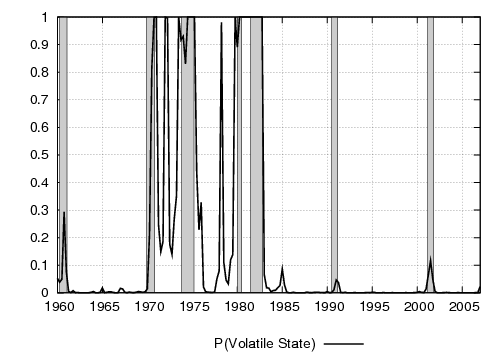
\includegraphics[scale=0.4]{results_re/states_sm.png} \\
    Expected 7.77 volatile years
  \end{center}
}

\frame
{
  \ft{Regime-Switching Volatility}
  \begin{center}
    Constant Gain Learning\\
    Probability Economy is in the Volatile Regime\\
    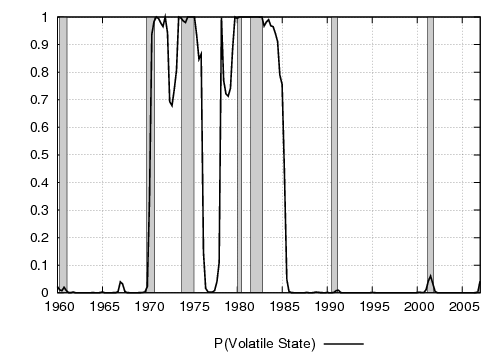
\includegraphics[scale=0.4]{results_cg_wlsinit/states_sm.png} \\
    Expected 12.26 volatile years
  \end{center}
}

\frame
{
  \ft{Regime-Switching Volatility}
  \begin{center}
    Dynamic Gain Learning\\
    Probability Economy is in the Volatile Regime\\
    and Evolution of the Learning Gain\\
    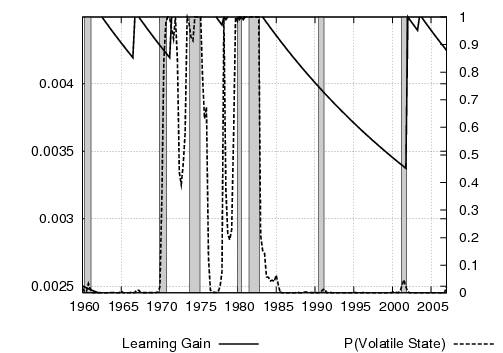
\includegraphics[scale=0.4]{results_dg8_wlsinit/states_sm.png} \\
    Expected 9.17 volatile years
  \end{center}
}

\subsection{Forecast Errors}

\frame
{
  \ft{Forecast Errors Comparison}
\tiny
  \begin{center}
\begin{tabular}{|l|c|c|c|}\hline
 & Rational Expectations & Dynamic Gain & Constant Gain \\ \hline 
RMSE Output Gap & 3.12 & 3.13 & 3.18 \\ 
RMSE Inflation & 4.41 & 4.69 & 4.69 \\ 
RMSE Federal Funds Rate & 5.01 & 5.05 & 5.09 \\ \hline 
AR(1) Output Variance & 0.0904 (0.0730) & 0.1715 (0.0722) & 0.1240 (0.0728) \\ 
AR(1) Inflation Variance & 0.1760 (0.0716) & 0.1364 (0.0699) & 0.1073 (0.0653) \\ 
AR(1) Fed Funds Variance & 0.3851 (0.0670) & 0.3798 (0.0659) & 0.3798 (0.0636) \\ \hline 
\end{tabular}
\end{center}
\normalsize
\bi
\item<+-> Rational Expectations actually (very slightly) fits data better than learning models.
\item<+-> All models show some persistence in volatility of forecast errors.
\item<+-> Models especially fail to explain changing volatility of the federal funds rate.
\ei
}

\frame {
  \ft{Forecast Errors: Output Gap}
  \begin{tabular}{ccc}
  Rational Exp. (1.0) & Constant Gain (0.86) & Dynamic Gain (0.82) \\
  \includegraphics[scale=0.18]{../badluck/results_re/output_err.png} &
  \includegraphics[scale=0.18]{../badluck/results_cg_wlsinit/output_err.png}  &
  \includegraphics[scale=0.18]{../badluck/results_dg8_wlsinit/output_err.png} \\
  \end{tabular}

  \bi
  \item (Correlation with Rational Expectations)
  \item All models made similar errors
  \item Most volatile during recessions in 1970s, early 1980s
  \ei
}

\frame {
  \ft{Forecast Errors: Inflation}
  \begin{tabular}{ccc}
  Rational Exp. (1.0) & Constant Gain (0.85) & Dynamic Gain (0.80) \\
  \includegraphics[scale=0.18]{../badluck/results_re/inflation_err.png} &
  \includegraphics[scale=0.18]{../badluck/results_cg_wlsinit/inflation_err.png}  &
  \includegraphics[scale=0.18]{../badluck/results_dg8_wlsinit/inflation_err.png} \\
  \end{tabular}

  \bi
  \item (Correlation with Rational Expectations)
  \item All models made similar errors.
  \item Most volatile during recessions in 1970s, early 1980s.
  \ei
}

\frame {
  \ft{Forecast Errors: Federal Funds Rate}
  \begin{tabular}{ccc}
  Rational Exp. (1.0) & Constant Gain (0.99) & Dynamic Gain (0.99) \\
  \includegraphics[scale=0.18]{../badluck/results_re/fedfunds_err.png} &
  \includegraphics[scale=0.18]{../badluck/results_cg_wlsinit/fedfunds_err.png}  &
  \includegraphics[scale=0.18]{../badluck/results_dg8_wlsinit/fedfunds_err.png} \\
  \end{tabular}

  \bi
  \item (Correlation with Rational Expectations)
  \item Essentially identical errors.
  \item Do not explain change in policy in early 1980s.
  \ei
}

\section{Conclusion}
\frame
{
  \ft{Conclusions}
  \bi
  \item<+-> When allowing for regime-switching volatility, there is little evidence of adaptive expectations.
  \item<+-> Constant gain learning and dynamic gain learning both produce less volatility for the natural rate shock.
  \item<+-> Learning frameworks actually deliver a higher prediction for the time spent in volatile regime.
  \item<+-> All models make similar forecast errors at similar points in sample.
  \item<+-> Rational expectations model actually yields smallest in-sample MSE.
  \ei
}



\end{document}

